\section{Experiment 10H-K: jointly learned plants and client memberships}
\label{sec:experiment10hk}

\paragraph{Question and predeclared design.}
Experiment 10H-J shows that releasing heuristic bounds does not validate a
single fleet plant: short prediction improves while longer propagation can
deteriorate. Experiment 10H-K tests whether two learned plants improve future
measured outputs under the same physical structure, covariance and bias
assumptions. Protocol commit \texttt{080a6aa} precedes fitting; implementation
commit \texttt{d5e1b11} is recorded in all ten execution manifests. The same
opened development fleets 601--605 contain 20 training and ten held-out
clients each. Confirmation 591--600 and 611--620 remains sealed.

Both component counts retain the eight positive coordinates, exact bicycle
coupling, coefficient box $[0.1,10]$, fixed public $R$, public $Q$ shape,
quiet-start bias correction and stationary-covariance/zero-state initialization
from 10H-I/J. The two fixed $Q$ scales, 0.01 and 1, are reported separately;
neither is selected here. The box remains a diagnostic domain, not a validated
engineering envelope. The audited 10H-J widest-box $K=1$ solutions and their
three-restart evidence are reused. Their output hashes, measured-array hashes
and training objectives are independently verified before $K=2$ fitting.

\paragraph{Joint plant--membership objective.}
For client $i$ and candidate plant $g$, let
\[
 D_{ig}=\sum_{j\in\mathcal R_i}\sum_t
 \left[e_{jgt}^{\mathsf T}S_{jg}^{-1}e_{jgt}
 +\log\det S_{jg}-\log\det R\right],
\]
where $\mathcal R_i$ contains every measured speed record associated with
that client. The models recompute $A_g(v),B_g(v)$, stationary covariance,
Kalman gain, innovations and their total derivatives at each proposal.
With $N$ record-time samples, the minimized objective is
\[
 L_K=-\frac{2}{3N}\sum_i\log\left(
    \sum_{g=1}^{K}\pi_g\exp[-D_{ig}/2]\right).
\]
Stable log-sum-exp gives the objective and current working membership weights.
For $K=1$ this is exactly the previous objective; duplicating its plant in
both components supplies an available nested reference. $K=2$ has sixteen
plant coordinates and one mixing weight, with $\pi_1\in[0.01,0.99]$ to keep
log weights finite. The limit does not force any hard client occupancy.
These weights are not calibrated class probabilities: covariance mismatch
and serial correlation established in 10H-I/J remain relevant.

Three deterministic random directions produce symmetric log-coordinate
perturbations of amplitude 0.3 around the learned global plant. Nearest
feasible projections retain exact coupling. No nominal-score clustering or
true class information initializes the models. Analytic-gradient SLSQP moves
both plants through actuator, relaxation and mechanics stages (80 iterations
each), then all seventeen variables jointly (800 iterations, tolerance
$10^{-12}$). Memberships evolve at every objective evaluation. The selected
restart minimizes training likelihood only.

\paragraph{Causal unseen-client validation.}
Only the first 50 samples, or 0.5\,s, of a held-out client's first listed speed
record determine its membership. That membership is frozen across all its
speed records. The primary deployment selects its maximum-weight component;
a secondary diagnostic averages separately propagated outputs with the same
fixed weights. No matrices or observer gains are interpolated, and no full
held-out score chooses a component.

All models, including the nominal reference, use common forecast origins
50--150 inclusive: 101 origins per 200-sample record, at horizons
1, 5, 20 and 50 samples. Filtered states use outputs strictly before each
origin; subsequent propagation uses known commands without intervening output
corrections. Separate zero-start simulations propagate from the record start
but score only samples 50--199, after membership calibration. Consequently
the $K=1$ errors here differ from the earlier full-record/20-sample-burn-in
tables despite identical fitted coefficients. Prediction and simulation
validate different aspects of an application model \cite{mathworksPrediction2026}.

\paragraph{Numerical and provenance result.}
All 30 independent $K=2$ restarts report success and satisfy KKT and feasibility
limits: maximum KKT residual $2.86\times10^{-6}$, zero constraint violation,
zero invalid fitting evaluations and coupling error $1.78\times10^{-15}$.
Every selected two-component training objective is below its global reference;
neither a collapsed reference nor a mixing-weight bound is selected.
Selected active-face Hessians have positive minimum eigenvalues, at least
0.00164. Training hard occupancy is at least seven clients per component at
$Q=0.01$ and six at $Q=1$.

One of ten predeclared finite-difference gradient checks narrowly misses the
$10^{-5}$ relative-error limit: seed 601, $Q=0.01$, has error
$1.14\times10^{-5}$ at step $10^{-5}$. At the unchanged initial point, steps
$5\times10^{-6}$ and $2.5\times10^{-6}$ give $2.84\times10^{-6}$ and
$7.81\times10^{-7}$, respectively. The approximately quadratic refinement
supports a finite-difference truncation explanation. The original missed
check remains recorded; no fit, criterion or protocol is changed.

An independent audit verifies all execution sources against committed
revision \texttt{d5e1b11}, all checkpoint hashes and unchanged historical gate
artifacts. The original single-model evaluator reproduces prefix memberships
to $4.13\times10^{-14}$ and independently computed component forecasts agree
to $2.10\times10^{-12}$. Six focused tests cover client aggregation, mixture
gradients and permutation invariance, first-record prefix isolation, forecast
equivalence, forecast causality and coupled feasibility. The full suite has
136 passing tests; all four new Python files pass scoped lint.

\paragraph{Fleet-average future-output result.}
Table~\ref{tab:10hk-prediction} and Figure~\ref{fig:10hk-fleet} show substantial
improvement beyond one-step filtering. The primary $K=2$ deployment improves
every reported horizon and suffix simulation relative to $K=1$ in all five
fleets, in both covariance panels. Mean paired training-objective improvement
is 35.14\% at $Q=0.01$ and only 1.31\% at $Q=1$; the latter still produces
large longer-horizon output gains. Working training likelihood and future
fixed-$R$ dynamics error measure different quantities.

\begin{table}[htbp]
\centering
\caption{Held-out output errors with frozen prefix-MAP memberships. Errors
are means across five fleets. Gains average the five paired fleet reductions,
not the ratio of the displayed means. All horizons share forecast origins.}
\label{tab:10hk-prediction}
\begin{tabular}{llrrr}
\toprule
$Q$ scale & Diagnostic & $K=1$ $E_R$ & $K=2$ $E_R$ & Paired gain (\%)\\
\midrule
0.01 & 0.01\,s forecast & 4.089 & 2.833 & 30.40\\
0.01 & 0.05\,s forecast & 12.664 & 7.089 & 43.51\\
0.01 & 0.2\,s forecast & 100.066 & 38.195 & 61.52\\
0.01 & 0.5\,s forecast & 165.009 & 49.796 & 70.07\\
0.01 & Zero-start suffix & 164.418 & 46.389 & 71.98\\
\midrule
1 & 0.01\,s forecast & 1.917 & 1.778 & 7.26\\
1 & 0.05\,s forecast & 7.673 & 4.534 & 40.81\\
1 & 0.2\,s forecast & 100.262 & 30.868 & 69.93\\
1 & 0.5\,s forecast & 228.686 & 61.572 & 73.31\\
1 & Zero-start suffix & 263.852 & 63.323 & 75.90\\
\bottomrule
\end{tabular}
\end{table}

At 0.5\,s, paired fleet gains range 63.13--74.75\% for $Q=0.01$ and
67.15--76.23\% for $Q=1$. Two-model forecasts and suffix simulations also
improve the public nominal reference in every fleet. The frozen-weight
ensemble gives similar results at $Q=0.01$, where prefix weights are almost
hard. At $Q=1$ it gives 74.40\% mean paired 0.5\,s gain, versus 73.31\%
for MAP; both predeclared rules are reported without selecting one afterward.

\begin{figure}[htbp]
\centering
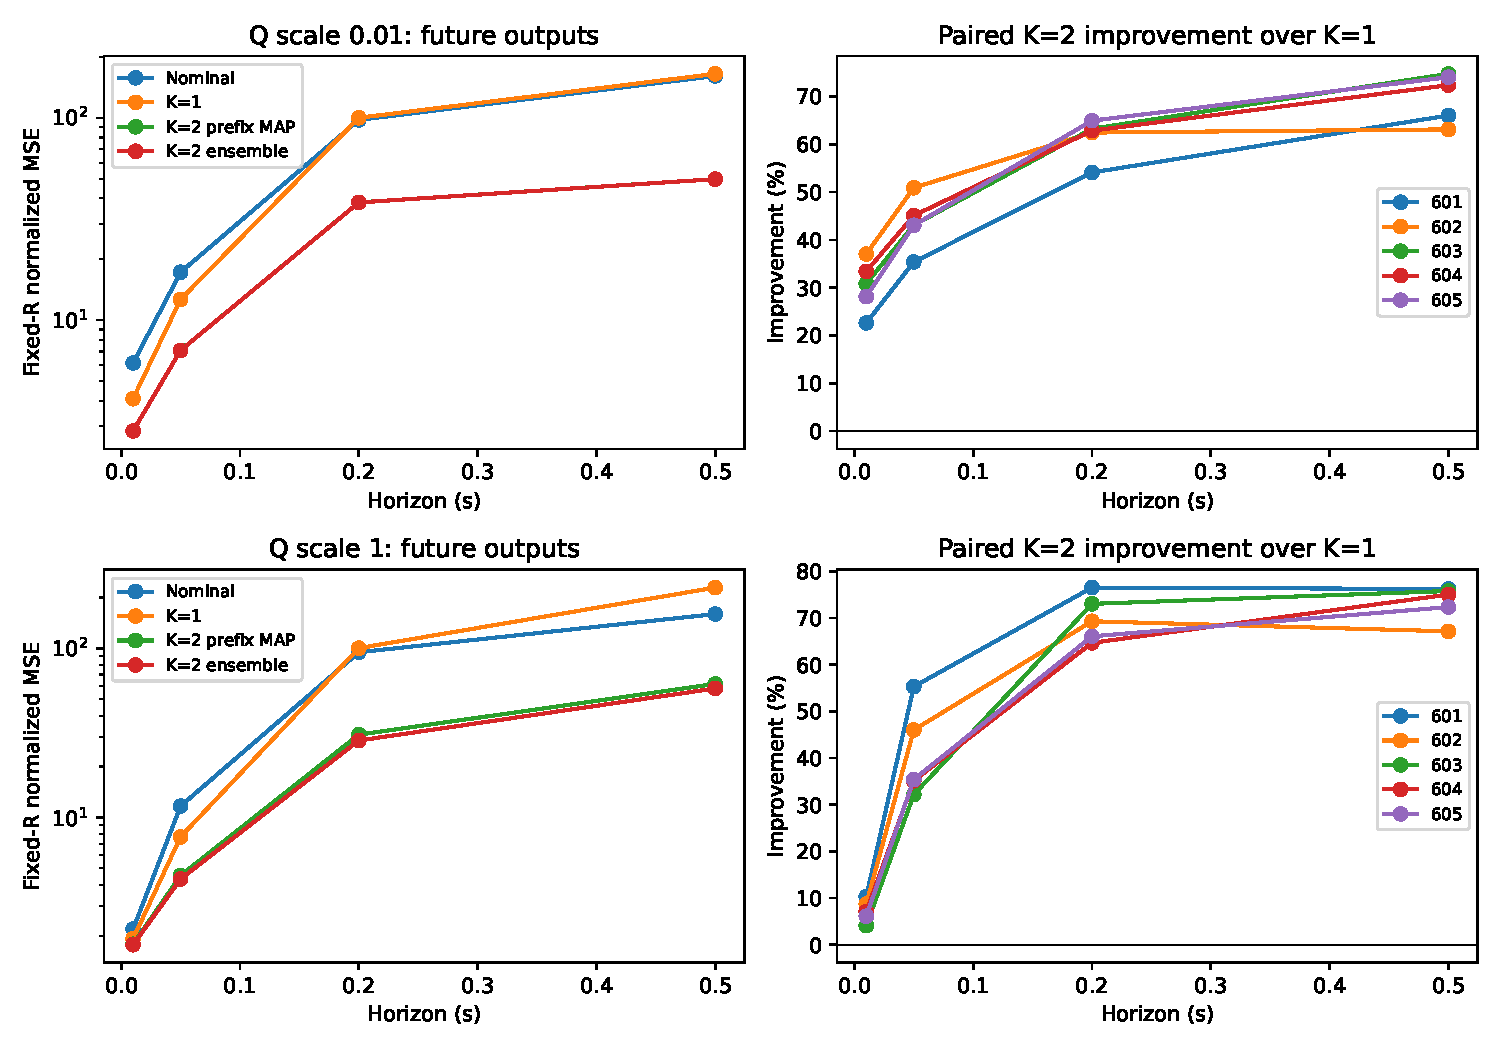
\includegraphics[width=\textwidth]{../results/figures/experiment_10hk_joint_client_mixture.pdf}
\caption{Future-output errors and paired fleet gains under the predeclared
calibration/forecast split. Every horizon is assessed without intervening
output corrections. Both fixed covariance panels and both deployment rules
are retained.}
\label{fig:10hk-fleet}
\end{figure}

\paragraph{Individual clients do not all benefit.}
Fleet-average improvement is not a universal personalization guarantee.
At 0.5\,s, 39/50 clients improve at $Q=0.01$ and 43/50 at $Q=1$.
Median client improvement is 73.64\% and 70.76\%, respectively. The worst
client error nevertheless increases by factors 14.06 and 3.71 relative to
$K=1$. At $Q=1$, for example, seed 602 client position 5 increases from
$E_R=22.56$ to 83.68. These positions are measured-record associations, not
vehicle class labels. Figure~\ref{fig:10hk-clients} exposes the unfavorable
tail. At $Q=0.01$, the arithmetic mean of client percentage gains is actually
$-16.47\%$ despite the 70.07\% mean paired fleet-error reduction: percentage
ratios place large weight on clients with small baseline errors. Both
aggregations must remain visible when deciding whether to deploy grouping.

\begin{figure}[htbp]
\centering
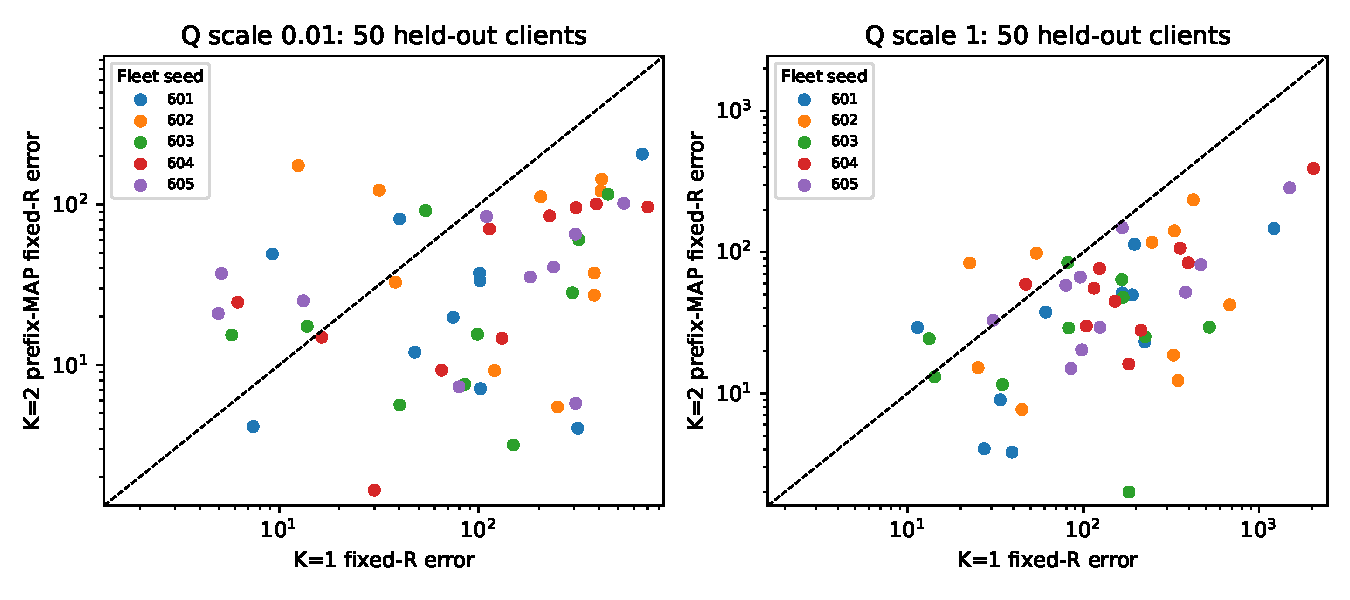
\includegraphics[width=\textwidth]{../results/figures/experiment_10hk_client_forecasts.pdf}
\caption{Per-client 0.5\,s fixed-$R$ errors. Points below the identity line
benefit from the two-model prefix-MAP deployment; points above it deteriorate.
All 50 held-out clients per panel are shown without class labels.}
\label{fig:10hk-clients}
\end{figure}

\paragraph{Model and partition repeatability remains unresolved.}
Numerical stationarity does not establish a unique two-model solution.
At $Q=0.01$, fleets 603--605 reproduce models and partitions across all three
starts; fleets 601 and 602 have minimum restart ARI 0.622 and 0.043 and
objective spreads 1.59\% and 9.67\%. ARI here compares learned partitions
with each other after fitting; it never compares them with true labels.
At $Q=1$, all five fleets have distinct stationary alternatives, despite
objective spreads only 0.17--0.27\%. Minimum restart ARI ranges
$-0.011$--0.799, and maximum aligned parameter CV ranges 0.387--1.051.
High working membership confidence therefore cannot certify a reproducible
physical grouping. No true family-count or class-recovery claim is made.

All five selected $Q=0.01$ mixtures retain one coefficient bound; at $Q=1$
four selected mixtures are interior and one reaches a rear-decay upper bound.
Exact coupling and interiority do not validate the broad engineering domain.
No physical confidence interval or calibrated client parameter is established.

\paragraph{Residual calibration remains unresolved.}
On the held-out suffixes, $Q=0.01$ changes mean normalized NIS from 3.373 to
2.393 and the mean fleet maximum within-record autocorrelation from 0.783 to
0.719. At $Q=1$, NIS changes from 0.433 to 0.407, while maximum
autocorrelation increases from 0.339 to 0.412. The corresponding mean
minimum/maximum whitened covariance eigenvalues are 0.171/0.681, below one.
Mean maximum past-input correlations fall from 0.315 to 0.249 and from
0.154 to 0.133, respectively, but remain present. These are descriptive
record-aware diagnostics, not independent-sample significance tests
\cite{mathworksResidual2026}. Two plants improve measured-output dynamics
without repairing the working noise model.

\paragraph{Consequence for the KF/controller learning story.}
This is positive development evidence for learning multiple compatible plant
models directly from measured outputs. The improvement persists when outputs
no longer correct the propagated state, supporting the plant-model part of
the proposed iterative learning loop. It is stronger evidence than nominal
score clustering or one-step error alone. The same learned $A_g(v),B_g(v)$
can supply plant dynamics to a KF and a controller, with their different
noise assumptions and control augmentations.

The result does not establish latent-state accuracy, calibrated memberships,
an acceptable worst-client outcome, a federated communication benefit or
closed-loop performance. Before an observer/controller deployment comparison,
the next development work should stabilize the mixture solutions, investigate
the covariance/objective mismatch and protect clients for whom specialization
degrades future prediction. A subsequent controlled closed-loop experiment
can separate observer-model and controller-model updates. Frozen-speed plant
poles and stationary KFs are not LPV/adaptive stability certificates. Historical
oracle/covariance gates remain unchanged, and confirmation remains unopened.

\paragraph{Reproducible artifacts.}
The protocol is \texttt{docs/experiment\_10hk\_protocol.md}; the execution
entry point is \texttt{experiment\_10hk\_joint\_client\_mixture.py} and the
independent reporting audit is \texttt{experiment\_10hk\_result\_audit.py}.
Results include all restart parameters and phases, initial splits, client
memberships, per-client/aggregate forecasts, residuals, refined gradient
checks and immutable source/output manifests under prefix
\texttt{results/tables/experiment\_10hk}. No labels, true client quantities,
latent trajectories or exact client matrices enter learning or this audit.
